\documentclass[12pt,a4paper]{article}
\usepackage[utf8]{inputenc}
\usepackage[english,lithuanian]{babel}
\usepackage[L7x]{fontenc}
\usepackage{lmodern}
\usepackage{amsmath}
\usepackage{amssymb}
\usepackage{theorem}
\usepackage{bm}
\usepackage{Sweave}
%\usepackage[unicode]{hyperref}
%\usepackage{ucshyper}
\pagestyle{plain}

\newcommand{\eps}{\varepsilon}
\newcommand{\E}{\mathbf{E}}
\newcommand{\PP}{\mathbf{P}}
\theoremstyle{change}\newtheorem{salyga}{Uždavinys}

\DeclareMathOperator{\spp}{sp}

\DeclareMathOperator{\Corr}{Corr}
\topmargin=0cm
\textheight=700pt
\textwidth=430pt
\oddsidemargin=0pt
\headsep=0pt
\headheight=0pt
%\voffset=-1in
\def\qed{\relax\ifmmode\hskip2em \Box\else\unskip\nobreak\hskip1em $\Box$\fi}








\begin{document}
\begin{titlepage}
\centerline{ \large VILNIAUS UNIVERSITETAS}
\bigskip
\centerline{\large MATEMATIKOS IR INFORMATIKOS FAKULTETAS}
\smallskip

\centerline{\large  EKONOMETRINĖS ANALIZĖS KATEDRA}
\vskip 200pt
\centerline{ \large Alina \textsc{Rauktytė} ir Povilas \textsc{Bočkus}}
\vskip 50pt
\centerline{\Large Ekonometrinis projektas}
\vskip 25pt
\centerline{\bf \Large \textsc{Darbo užmokesčio nustatymo mechanizmas}}
\vskip 25pt
\bigskip
\vskip 50pt
\begin{flushright}
 Kursinio projekto vadovas: 
 doc. Remigijus Lapinskas
\end{flushright}
\hfill Ekonometrija, III kursas, 2 grupė
\vskip 150pt
\centerline{\large VILNIUS 2011}
\end{titlepage}

\tableofcontents
\pagebreak







\section{Įvadas}
\bigskip
\hspace{40pt}Atlyginimų reikšmė šalies ekonomikoje yra neabejotinai didelė. Todėl šiandien darbo užmokestis yra vienas svarbiausių ekonominių tyrimų objektų. Ekonomistus domina, kas ir kokiu būdu lemia darbo užmokesčio pasikeitimus trumpuoju ir ilguoju laikotarpiais, kokiais sąryšiais jis susijęs su kitais ekonominiais rodikliais.
\vskip 8pt
$\qquad $Atsižvelgiant į tai, kad darbdaviai ir darbuotojai paprastai pasirašo ilgalaikes darbo sutartis,  kuriose nustatomas darbo užmokestis, išryškėja viena pagrindinių atlyginimo savybių – lėta reakcija į ekonomikos pasikeitimus. Į visa tai turi būti atsižvelgta interpretuojant įvairius ekonomitrinės analizės rezultatus.
\vskip 8pt
$\qquad $Daugelis ekonomikos teorijoje pasiūlytų darbo užmokesčio modelių aprašo atlyginimą mikroekonominiame lygmenyje. Pagrindinis šio darbo tikslas yra atrasti geriausiai Lietuvos duomenis aprašantį modelį, t.y. tokį modelį, kuris apimtų bendrą vidutinį Lietuvos atlyginimą. Duomenys, su kuriais dirbome, be darbo užmokesčio, apima ir tokius pagrindinius Lietuvos ekonomikos rodiklius kaip bendras vidaus produktas, kainų lygis ir kt.
\vskip 8pt
$\qquad $Šio darbo ekonometrinė analizė sudaryta iš dviejų dalių.  Pirmoje dalyje nagrinėjame autoregresinį modelį, aprašantį laikinę darbo užmokesčio seką. Su galutiniu modeliu pateiksime prognozę. Antra dalis apima paklaidų korekcijos modelio analizę. Pirmiausia nagrinėsime modelį, neįtraukiant darbo našumo, vėliau vertinsime modelio tikslumo pokyčius, į modelį įtraukiant darbo našumą.
\vskip 8pt
\pagebreak









\section{Darbo užmokestis}
\bigskip



\subsection{Darbo rinka}
\medskip
\hspace{40pt}Darbo užmokestis yra piniginis atlyginimas už darbinę veiklą. Jis apibrėžia bendrą šalies gyvenimo lygį, visos ekonomikos gerovę ir daro didelę įtaką žmonių kasdieniam gyvenimui. Tai pagrindinė ekonomiškai aktyvių žmonių pajamų dalis. Dauguma pensijų ir pašalpų sistemų yra pagrįsti darbo užmokesčio lygių analize ir dinamika. Taigi, darbo užmokestis lemia žmonių pajamų dydį. Pajamos lemia vartojimą, todėl darbo užmokestis glaudžiai su juo susijęs.
\vskip 8pt
$\qquad $Darbo užmokestis dažnai yra viena pagrindinių įmones gaminamos produkcijos sąnaudu komponenčiu. Sąnaudos yra kainų pagrindas, taigi darbo užmokesčio pasikeitimai yra vienas svarbiausių veiksnių lemiančių kainų pasikeitimą. Vadniasi, atlyginimai atlieka itin svarbų vaidmenį ekonomikoje.
\vskip 8pt
$\qquad $Darbo užmokestis gali būti nustatomas daugeliu būdų. Vienas iš jų - kolektyvinės derybos, kuomet susitarimas dėl darbo užmokesčio pasiekiamas derantis įmonėms ir profsąjungoms. Kita darbo užmokesčių dalis nustatoma darbdavių valia, arba susitarimu tarp darbdavio ir darbuotojo. 
\vskip 8pt
$\qquad $Klasikinio modelio šalininkai teigia, jog atlyginimą - darbo kainą – apibrėžia pasiūla ir paklausa. Darbo užmokesčio dydį lemia pasiūlos veiksnys – skaičius žmonių, kurie yra pasiruošę pradėti dirbti, ir paklausos veiksnys – reikalingų darbo rinkoje darbuotojų skaičius. Mikroekonominiame lygmenyje darbo užmokestį apibrėžia darbuotojų kvalifikacija, gebėjimai bei užimamos pareigos. Visi minėti faktoriai ir sąveika tarp jų suformuoja darbuotojo ir darbdavio susitarimą, kuriuo apibrėžiamas darbo užmokestis. 
\vskip 8pt
$\qquad $Jeigu darbo rinkoje darbdaviai negali rasti pakankamai darbuotojų, atitinkančių jų reikalavimus, darbdaviai atlyginimą kels iki tokio lygio, kuris privilios aukštesnės kvalifikacijos darbuotojus. Ir atvirkščiai, jei darbo rinkoje darbuotojų pasiūla yra perteklinė, tai darbo užmokestis kris. Kai pasiūla lygi paklausai, susidaro pusiausvyros darbo užmokesčio lygis. Paveiksle Nr.1, tokį lygį atitinka w* darbo rinkos pusiausvyros taške A. 
\vskip 8pt

\begin{center}
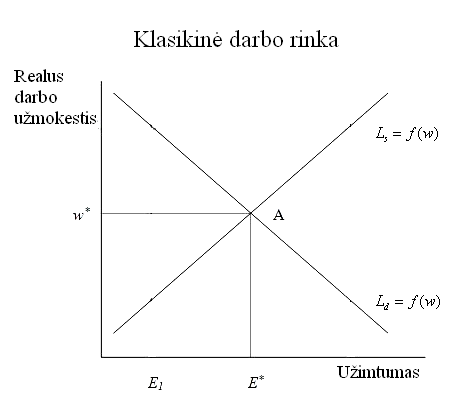
\includegraphics[width=80mm,height=60mm]{darborinka.PNG}
\\
\textit{Paveikslas Nr.1}
\end{center}

\vskip 8pt
$\qquad $Sumažėjusi bendroji paklausa, didina nedarbą. Klasikinis modelis aprašo ilgojo laikotarpio pusiausvyrą, kuomet ekonomika derinasi prie pasikeitusių aplinkybių. Tačiau darbo užmokesčio kaita yra ypatingai lėtai, todėl ekonomikos prisiderinimas prie naujos pusiausvyros dažniausiai yra lėtas. Panagrinėsime, kodėl darbo užmokestis keičiasi lėtai.
\vskip 8pt
$\qquad $Darbas yra ilgalaikė sutartis tarp darbuotojo ir darbdavio. Tokia sutartis yra naudinga abiems šalims. Kai firma atleidžia darbuotoją, ji netenka jo turėtos darbo patirties, darbo metu įgytų žinių ir įgūdžių. Naujo darbuotojo samdymas sudaro papildomus kaštus jo apmokymui, įskaičiuojant prarastą laiką, darbuotojo adaptacijai naujoje darbo vietoje. Firma vengia atleisti senus darbuotojus esant gamybos pokyčiams, tikėdamiesi, jog šie pokyčiai yra trumpalaikiai. 
\vskip 8pt
$\qquad $Ilgalaikė sutartis taip pat naudinga ir darbuotojams. Atleistasis iš darbo praranda darbo užmokestį ir dažniausiai turi pasirengti ilgoms, nemažų pastangų reikalaujančioms, naujo darbo paieškoms. Darbo sutartimi dažniausiai patvirtinamas dviejų šalių kompromisas dėl darbo užmokesčio, jo dydžio svyravimo, kintant gamybos apimtims.
\vskip 8pt
$\qquad $Darbo užmokesčio prisiderinimas prie darbo rinkos pokyčių ir reikalavimų yra lėtas, nes ilgalaikės darbo sutartys sudaro galimybę firmoms ir jų darbuotojams izoliuotis nuo darbo rinkos sąlygų. Taigi, vykstant darbo rinkos ir visos ekonomikos pokyčiams, atsiradus žymiems nuokrypiams nuo darbo rinkos pusiausvyros, darbo užmokestis reaguoja palyginti lėtai. Todėl analizuojant atlyginimų ir ekonomikos faktorių sąveiką būtina atsižvelgti į laiką, reikalingą darbo užmokesčio prisiderinimui prie naujos pusiausvyros.
\vskip 8pt



\subsection{Ekonominiai modeliai}
\medskip
\hspace{40pt} Kaip jau buvo minėta, vienas pagrindinių ekonomikos tikslų, analizuojant darbo užmokestį, yra nustatyti jo priklausomybę nuo įvairių ekonomikos rodiklių. Ekonomikos teorijoje yra pasiūlyta nemažai darbo užmokestį nusakančių modelių, leidžiančių ne tik įžvelgti santykį tarp kintamųjų, bet ir numatyti artimiausias tendencijas. Pateiksime keletą modelių, tam kad galėtume juos palyginti ir nustatyti gaires, padėsiančias šio darbo eigoje rasti tinkamiausią modelį.
\vskip 8pt

\small { \textit{Fregert modelis}:}
\begin{center}
\large $ \Delta w=\beta_0+\beta_1(\frac{w_{t-1}}{w_{agg}})+\beta_2u_t+\beta_3\pi_t+\varepsilon_t $
\end{center}
\vskip 8pt
$\qquad $Šiame modelyje darbo užmokesčio pokytis paaiškinamas darbo užmokesčio ankstiniu, padalintu iš visuminio darbo užmokesčio, vienalaikiais nedarbo lygiu ir infliacija. Šis modelis nagrinėja individualų darbo užmokestį, tačiau duoda informacijos apie atlyginimo priklausomybę nuo kitų kintamųjų. Tai labai apibendrintas modelis, palyginti su Nymoen modeliu.
\vskip 8pt

\small { \textit{Nymoen modelis}:}
\begin{center}
\large $ \Delta w=\beta_0+\beta_1\Delta p_t+\beta_2\Delta n_t+\beta_3(w_{t-1}-p_{t-1}-n_{t-1})+\beta_4 u_{t-1}+\varepsilon_t$
\end{center}
\vskip 8pt
\hspace{40pt}Nymoen atlyginimo pokytį aiškina kainų pokyčiu, našumo pokyčiu, nedarbo lygio ankstiniu, ir sudėtiniu nariu, į kurį įeina darbo užmokestis, našumas ir kainos. Kintamųjų ankstiniai patvirtina anksčiau aptartus ekonominius samprotavimus, jog darbo užmokestis ne iš kart reaguoja į kitų rodiklių pokyčius. 
\vskip 8pt
$\qquad $Vienas populiariausių atlyginimą apibūdinančių modelių yra darbo užmokesčio nustatymo mechanizmas ir kainų nustatymo mechanizmas. Darbo užmokestis šiame modelyje priklauso nuo laukiamo kainų lygio, nedarbo lygio ir abstraktaus kintamojo, kuris įvardija veiksnius, galinčius paveikti darbo užmokestį. Remiantis šiuo modeliu, darbo rinkos pusiausvyra reikalauja, kad darbo užmokestis, nustatytas pagal darbo užmokesčio nustatymo mechanizmą, būtų lygus darbo užmokesčiui, nulemtam kainų nustatymo mechanizmo. Šio modelio pusiausvyra pavaizduota paveiksle Nr. 2.
\vskip 8pt

\begin{center}
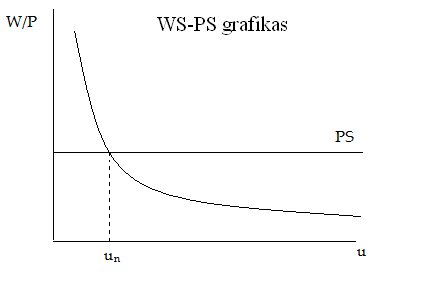
\includegraphics[width=80mm,height=60mm]{wsps.PNG}
\\
\textit{Paveikslas Nr.2}
\end{center}

\vskip 8pt
$\qquad $Apibendrinant, galime padaryti išvadą, kad darbo užmokestis, arba jo pasikeitimai, priklauso nuo infliacijos lygio, nedarbo lygio, darbo užmokesčio ankstinio, kainų lygio, darbo našumo. Į visa tai atsižvelgsime ieškodami tinkamiausio modelio, aprašančio Lietuvos darbo užmokestį.

\pagebreak









\section{Duomenų analizė}
\bigskip





\subsection{Duomenų aprašymas}
\medskip
\hspace{40pt}Ankstesniame skyriuje apžvelgėme nuo ko priklauso darbo užmokestis. Remiantis šiais ekonominiais samprotavimais, mūsų tyrimui reikės tokių duomenų (šaltinis http://www.stat.gov.lt/lt/):

\medskip

\begin{itemize}
\item Vidutinis nominalusis atlyginimas (wage);
\item Darbo jėga (l);
\item Darbuotojų skaičius (e);
\item Vartotojų kainų indeksas (p);
\item Bendras vidaus produktas (y).
\end{itemize}

Visi aukščiau minėti duomenys yra nuo 2000-ųjų metų pirmojo ketvirčio iki 2008-ųjų metų ketvirto ketvirčio imtinai. Skliaustuose nurodyti kintamųjų pavadinimai, kuriuos naudojome atliekant analizę R programa. 
\vskip 8pt
$\qquad $Dauguma ekonominių modelių aprašo atlyginimą mikroekonominiame lygmenyje. Šio kursinio pagrindinis tikslas yra atrasti visuminio šalies darbo užmokesčio priklausomybę nuo kitų kintamųjų.
\vskip 8pt
$\qquad $Kaip matysime vėliau, visi duomenys turi daugiau mažiau eksponentinį augimą. Aprašant sąryšius tarp skirtingų kintamųjų būtų sudėtinga interpretuoti rezultatus, nes duomenys auga eskponentiškai, jų augimo greičiai skiriasi. Todėl sudarinėjant modelius, naudosime šių duomenų logaritmus, t.y. duomenų augimas „maždaug“ atitiks tiesę. Sąryšius tarp tokių duomenų intepretuoti kur kas paprasčiau. Dar vienas logaritmuotų duomenų privalumas – logaritmuotų duomenų skirtumas atitinka procentinį pokytį.
\vskip 8pt
$\qquad $Toliau trumpai aptarsime kintamuosius atskirai. 






\subsubsection{Nominalusis atlyginimas}

\hspace{40pt}Nominalieji Lietuvos darbuotojų atlyginimai buvo gauti kaip trijų sektorių vidutinių atlyginimų vidurkis, t.y. kiekvienų metų ketvirčio, pradedant nuo 2000 – ųjų pirmojo ketvirčio ir baigiant 2008 – ųjų ketvirtu ketvirčiu, šalies ūkio be individualių įmonių, valstybės sektoriaus ir privataus sektoriaus be individualių įmonių atlyginimų bendras vidutinis atlyginimas.
\vskip 8pt
$\qquad$ Mus domina, kokia yra Lietuvos atlyginimų tendencija laiko atžvilgiu. Pateikiame nominalaus atlyginimo grafiką:
\vskip 8pt
\begin{center}
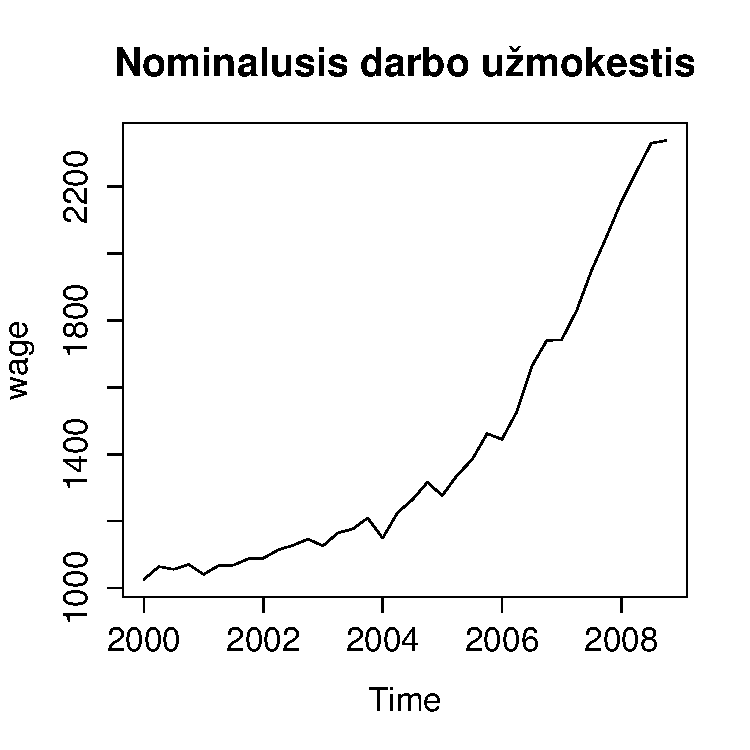
\includegraphics[width=70mm,height=70mm]{nwage}
\end{center}
Matome darbo užmokesčio kilimo tendenciją, išskirčių nėra. Turimi duomenys neįtraukia krizės laikotarpio, todėl nematome  numanomo atlyginimų sumažėjimo.  
\vskip 8pt







\subsubsection{Darbo jėga, dirbančiųjų skaičius, užimtumo lygis}

\hspace{40pt} Darbo jėga - tai visi dirbantys ir aktyviai ieškantys darbo šalies piliečiai, kitaip tariant, žmonės, kurie nori ir gali dirbti, ir kurie dirba. Duomenyse darbo jėga matuojama tūkstančiais. 
\vskip 8pt
\begin{center}
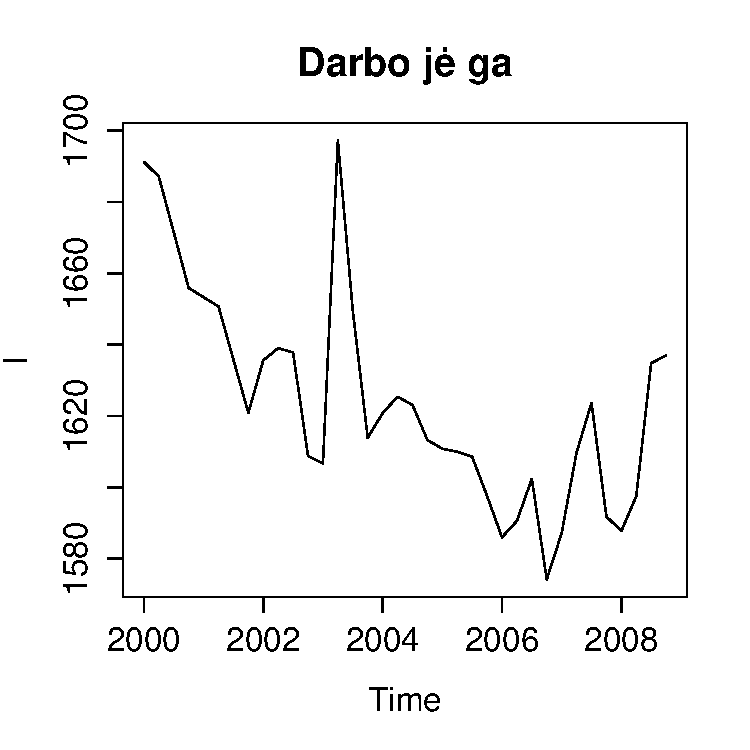
\includegraphics[width=70mm,height=70mm]{l}
\end{center}
Grafike matoma  darbo jėgos mažėjimo tendencija, bei sezoniškumas.
\vskip 8pt
$\qquad$Dalį darbo jėgos mažėjimo galime paaiškinti padidėjusiu emigrantų skaičiumi – didelės darbo jėgos dalies išvykimu iš šalies. Kita darbo jėgos mažėjimo priežastis galėtų būti viltį praradusių žmonių skaičiaus didėjimas. Tai žmonės, kurie nustojo ieškoti darbo. Jie jau nebeįskaičiuojami į darbo jėgą, taigi ji mažėja. 
\vskip 8pt
$\qquad$Dirbantieji – tai žmonės, kurie turi darbą. Dirbančiųjų skaičius mūsų duomenyse matuojamas tūkstančiais. Iš  grafiko matome, jog bendra dirbančiųjų skaičiaus tendencija yra didėjanti, tačiau šie duomenys pasižymi gana dideliais svyravymais.
\vskip 8pt
\begin{center}
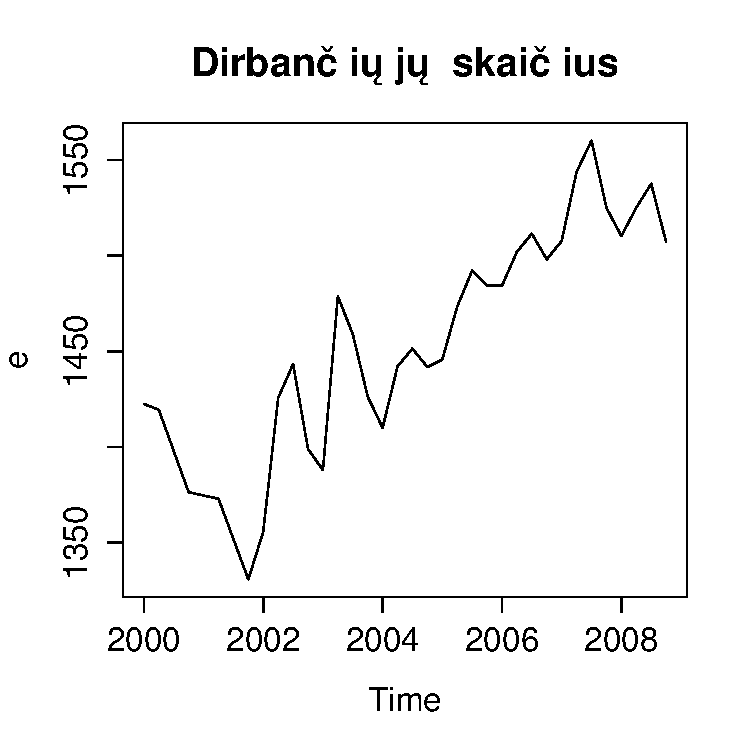
\includegraphics[width=70mm,height=70mm]{e}
\end{center}
\vskip 8pt
$\qquad$Taip pat vienas svarbesnių rodiklių apibūdinančių darbo užmokestį yra užimtumo lygis. Grafike matyti, kad užimtumas Lietuvoje nuo 2000 iki 2007 metų auga, tačiau tolesniu laikotorapiu ima kristi. Užimtumo lygį žymėsime \textit{er}. 
\begin{center}
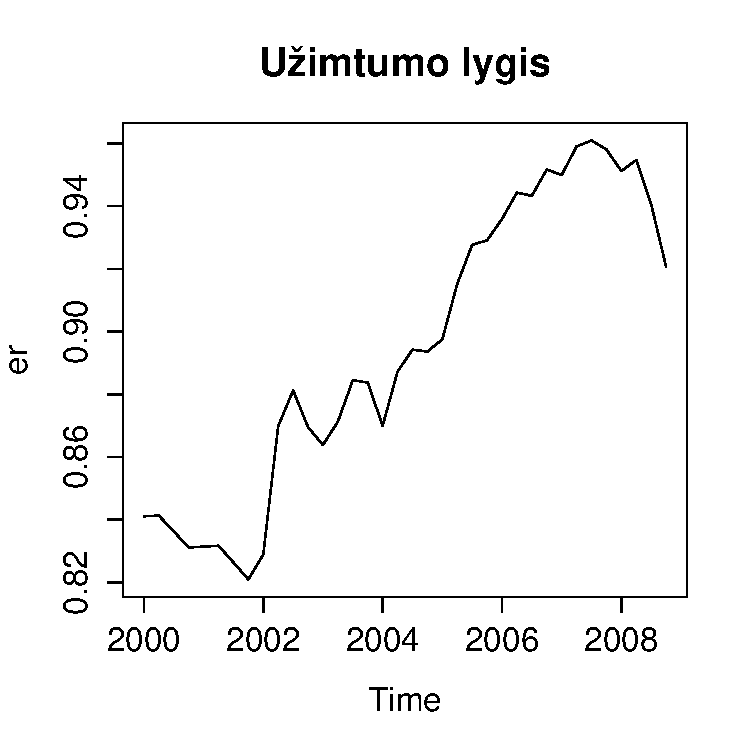
\includegraphics[width=70mm,height=70mm]{er}
\end{center}



\subsubsection{Vartotojų kainų indeksas}

\hspace{40pt}Kainų indekso baziniu laikotarpiu pasirinkti 2005 m. Matome aiškią kainų kilimo tendenciją. Nuo 2000 metų iki 2004 metų kainų indeksas gana stabilus palyginti su kainų indekso elgesiu nuo 2004 metų,- nuo to laikotarpio kainų indekso kilimo greitis didėja. 
\vskip 8pt
\begin{center}
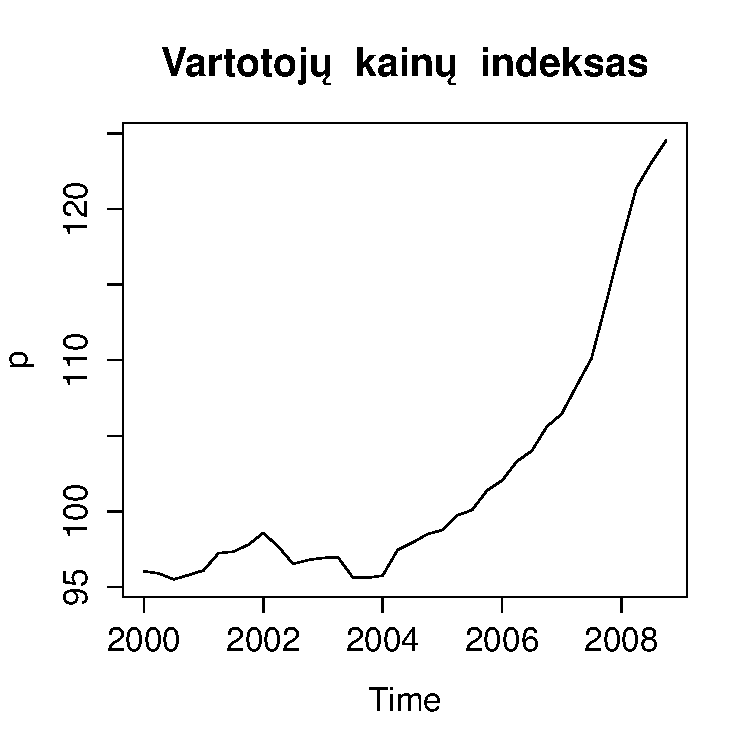
\includegraphics[width=70mm,height=70mm]{p}
\end{center}







\subsubsection{Bendras vidaus produktas ir našumas}

\hspace{40pt}Nominalusis bendras vidaus produktas matuojamas milijonais. 
\vskip 8pt
\begin{center}
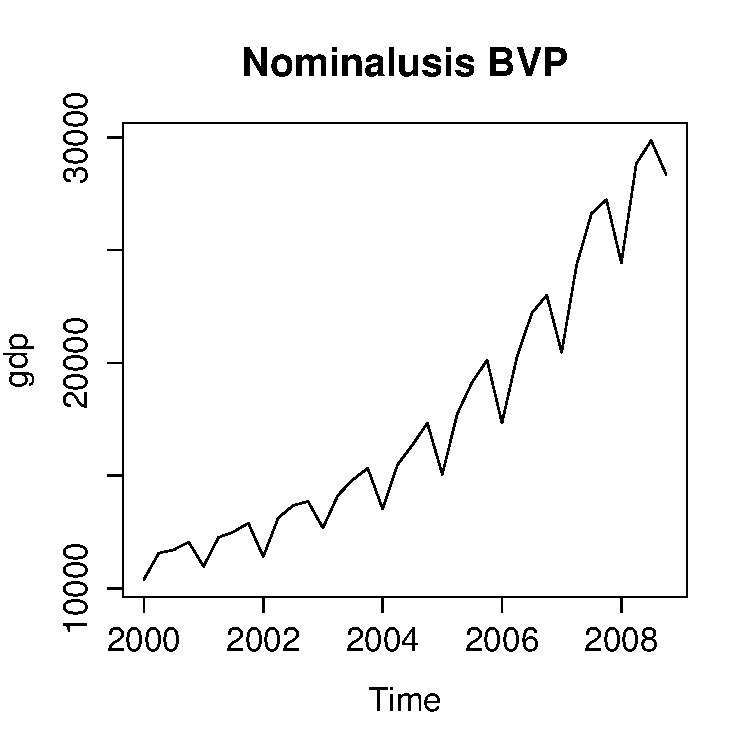
\includegraphics[width=70mm,height=70mm]{ngdp}
\end{center}
Iš grafiko matome kilimo tendenciją, bei gana ryškų duomenų sezoniškumą, todėl sezoniškumą elinimavome. Sutvarkyti duomenys pavaizduoti grafike. 
\vskip 8pt
\begin{center}
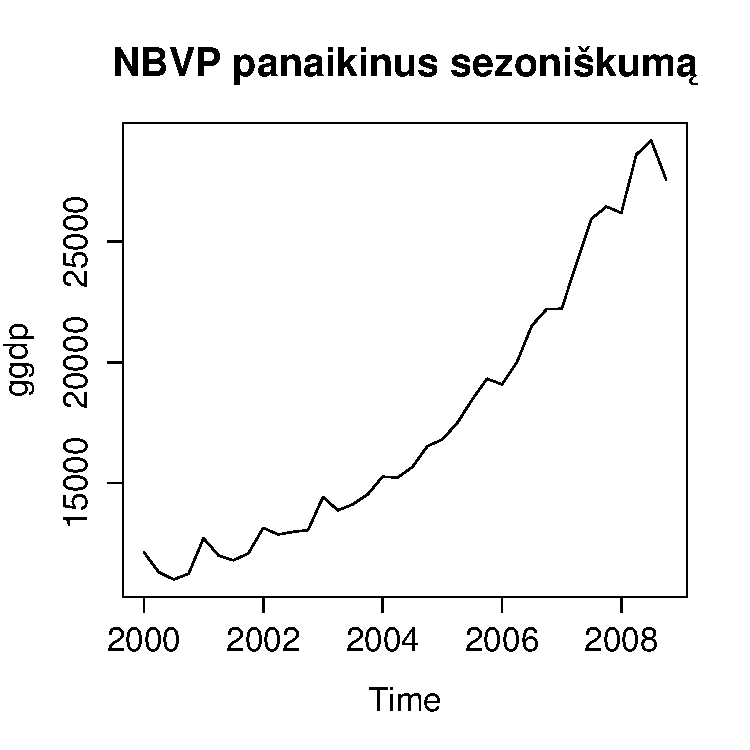
\includegraphics[width=70mm,height=70mm]{gngdp}
\end{center}
\vskip 8pt
$\qquad$Darbo našumas taip pat yra vienas iš svarbiausių rodiklių apibūdinančių darbo užmokestį. Jis buvo apskaičiuotas  bendrajį vidaus produktą padalinant iš dirbančiųjų skaičiaus. Darbo našumą žymėsime \textit{n}. Logiška, kad kuo žmonės našiau dirba, tuo didesnį darbo užmokestį gauna. Grafike galime pastebėti didėjančią darbo našumo tendenciją. 

\begin{center}
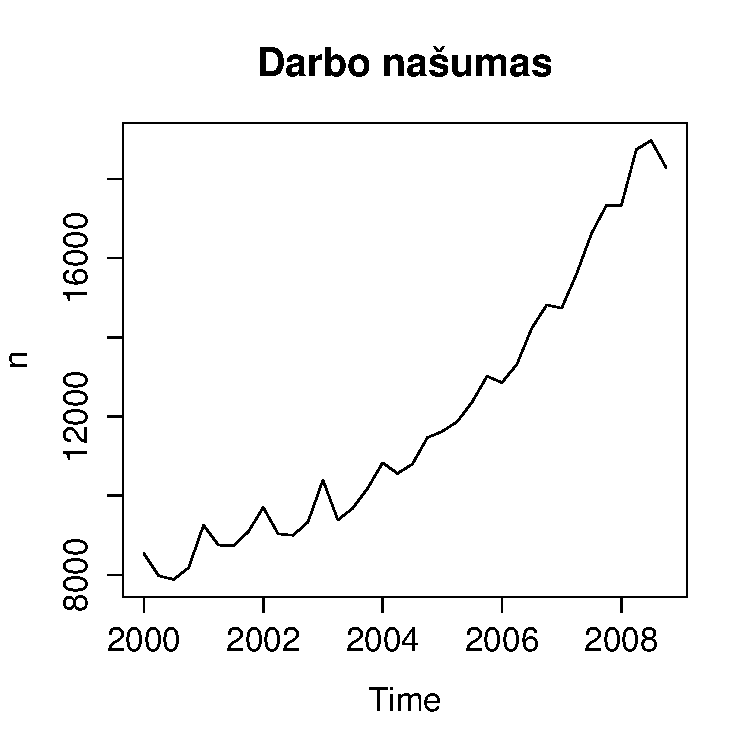
\includegraphics[width=70mm,height=70mm]{nn}
\end{center}
\vskip 8pt








\subsection{Kintamųjų vienetinių šaknų tyrimas}
\medskip


\hspace{40pt}Vienetinės šaknies egzistavimo tyrimas reikalingas tam, kad galėtume tinkamai sudaryti kointegracijos modelį. Išsiaiškinsime, ar mūsų logaritmuoti duomenys turi vienetinę šaknį. Visiems logaritmuotam kintamiesiems, kuriuos naudosime sudarant modelius, pritaikėme \textit{ur.df} funkciją norėdami ištirti vienetinės šaknies egzistavimą. Žemiau pateikiama lentelė su kiekvieno kintamojo statistikomis, gautomis \textit{ur.df} testu (kai $\alpha =0.05 $, kritinė reikšmė lygi –3.5).

\vskip 15pt

\begin{center}
\begin{tabular}{|c|c|}
\hline\textbf{ Kintamasis} &\textbf{ t - stat. reikšmė }\\ 
\hline log(wage) & -1.5776 \\ 
\hline log(p) & -0.0441 \\ 
\hline log(er) & -0.3865 \\ 
\hline log(n) & -3.0433 \\ 
\hline 
\end{tabular} 
\end{center}
Kadangi visos t-statistikų reikšmės viršija kritinę reikšmę, nulinės hipotezės, kad egzistuoja vienetinė šaknis kiekviename iš kintamųjų, neatmetame. 

\pagebreak









\section{Ekonometrinio modelio sudarymas}
\bigskip





\subsection{Autoregresiniai modeliai}
\medskip
\hspace{40pt}Paprastai kalbant, autoregresiniu modeliu aprašomos sekos, kurios turi atminties savybę. Tiksliau, autoregresinis modelis eilės p, žymimas AR(p), apibrėžiamas taip: 
\begin{center}
\large $ X_t=c+\sum\limits_{i=1}^{p}\varphi_i X_{t-i}+\varepsilon_t $
\end{center}
kur $ \varphi_1,..,\varphi_p $ yra modelio parametrai, $ c $ yra konstanta ir $ \varepsilon_t $ yra baltasis triukšmas.
\vskip 8pt
$\qquad$Remiantis ekonominiais samprotavimais, darbo užmokesčio dydžio nustatymas laikotarpiu t turėtų priklausyti nuo laikotarpiu t-1 nustatyto darbo užmokesčio, kuris vėlgi  priklauso nuo t-2 laikotarpio darbo užmokesčio ir t.t. Taigi, praeitų laikotarpių darbo užmokesčiai su tam tikru svoriu daro įtaką šio laikotarpio atlyginimui. Atmetus kitus galimus ekonominius faktorius, kurie gali turėti įtakos kintamajam \textit{wage}, sudarysime autoregresinį modelį, geriausiai aprašantį mūsų turimus duomenis.
\vskip 8pt
$\qquad$ Dauguma metodų, kurie įvertina autoregresinio modelio parametrus, remiasi prielaida, jog seka yra stacionari. Praeitame skyriuje įsitikinome, jog darbo užmokestis turi vienetinę šaknį. Jei nepaisytume šio fakto, sudarę modelį, gautume tariamąją regresiją (\textit{angl.} spurious regression). Tačiau darbo užmokesčio skirtumai yra stacionarūs, todėl juos ir naudosime.
\vskip 8pt



\subsubsection{Autoregresinio modelio sudarymas}
\hspace{40pt}Pirmiausia pasinaudojome programos R funkcija \textit{auto.arima} iš \textit{forecast }paketo. Ši funkcija siūlo geriausiai duomenis aprašantį ARIMA modelį, remdamasi adekvatumo kriterijų AIC, AICc arba BIC reikšmėmis. Remiantis \textit{auto.arima}, turimus duomenis geriausiai aprašo modelis skirtumams, t.y. ARIMA(0,1,0), pavidalo
\begin{center}
\large $  \log wage_t=c+\log wage_{t-1}+\varepsilon_t$
\end{center}
\vskip 8pt
$\qquad$Tačiau toks modelis atrodo sunkiai suderinamas su ekonominiais samprotavimais. Jau minėjome, jog darbo užmokesčio reakcija į įvairius ekonominius pokyčius yra gana lėta. Taigi, atlyginimo dydžio priklausymas nuo atlyginimo, nustatyto prieš tris mėnesius, atrodo šiek tiek įtartinas.
\vskip 8pt
$\qquad$Remdamiesi žemiau pateiktu laikinių sekų išskaidymo pagal ACF ir PACF grafiku, galime daryti prielaidą, jog darbo užmokesčio logaritmų skirtimų seka yra ketvirtos eilės AR modelis. 
\vskip 8pt

\begin{center}
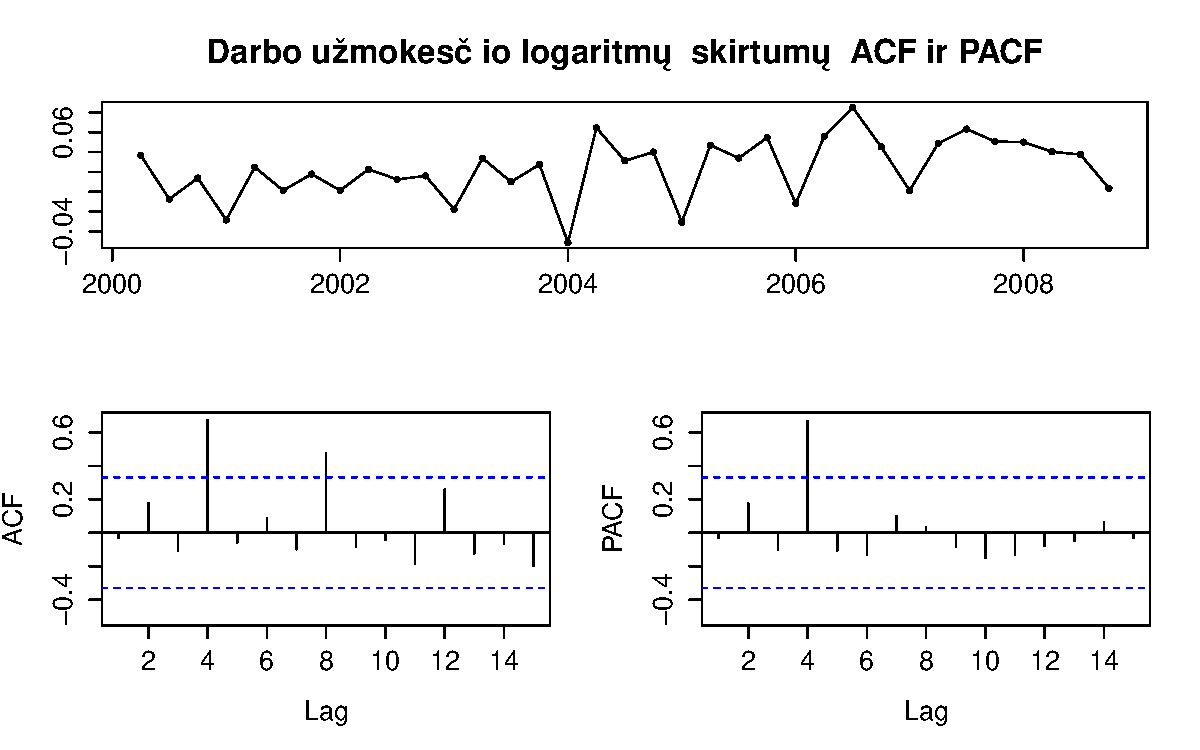
\includegraphics[width=100mm,height=70mm]{pacf}
\end{center}
\vskip 8pt
$\qquad$Sudarome 4 eilės AR modelį darbo užmokesčio logaritmų skirtumams:

\begin{center}
\large$ \Delta\log wage_t=\alpha+\beta_1\Delta\log wage_{t-1}+\beta_2\Delta\log wage_{t-2}+\beta_3\Delta\log wage_{t-3}+\beta_4\Delta\log wage_{t-4} +\varepsilon_t$ 
\large\\ $ \Updownarrow $
\large\\$ \log wage_t=\alpha+\log wage_{t-1}+\beta_1\Delta\log wage_{t-1}+\beta_2\Delta\log wage_{t-2}+\beta_3\Delta\log wage_{t-3}+\beta_4\Delta\log wage_{t-4}+\varepsilon_t $ 
\end{center}
Šis modelis atsižvelgia į ekonomikos teoriją. Jis aprašo darbo užmokesčio priklausomybę nuo darbo užmokesčio, nustatyto prieš metus. 
\vskip 8pt
$\qquad$Taigi, lyginant pastarąjį modelį su modeliu, kurį siūlė funkcija \textit{auto.arima}, galime padaryti išvadą, jog modelis logaritmuotiems darbo užmokesčio skirtumams AR(4) yra priimtinesnis, nes:

\begin{itemize}
\item dėl ilgalaikių darbo sutarčių ir lėtos reakcijos į ekonomikos pokyčius, darbo užmokestis turėtų priklausyti nuo ankstesnio darbo užmokesčio;
\item antrojo  modelio AIC yra mažesnis už pirmojo modelio;
\item grafiškai modeliuojamos reikšmės (raudona spalva) geriau atitinka faktines reikšmes (juoda spalva) darbo užmokesčio logaritmų skirtumo AR(4) modelio atveju (paveikslas Nr.3) palyginus su \textit{auto.arima} siūlomu ARIMA(0,1,0) modelio reikšmėmis (paveikslas Nr.4).
\end{itemize}
\vskip 8pt   

\begin{center}
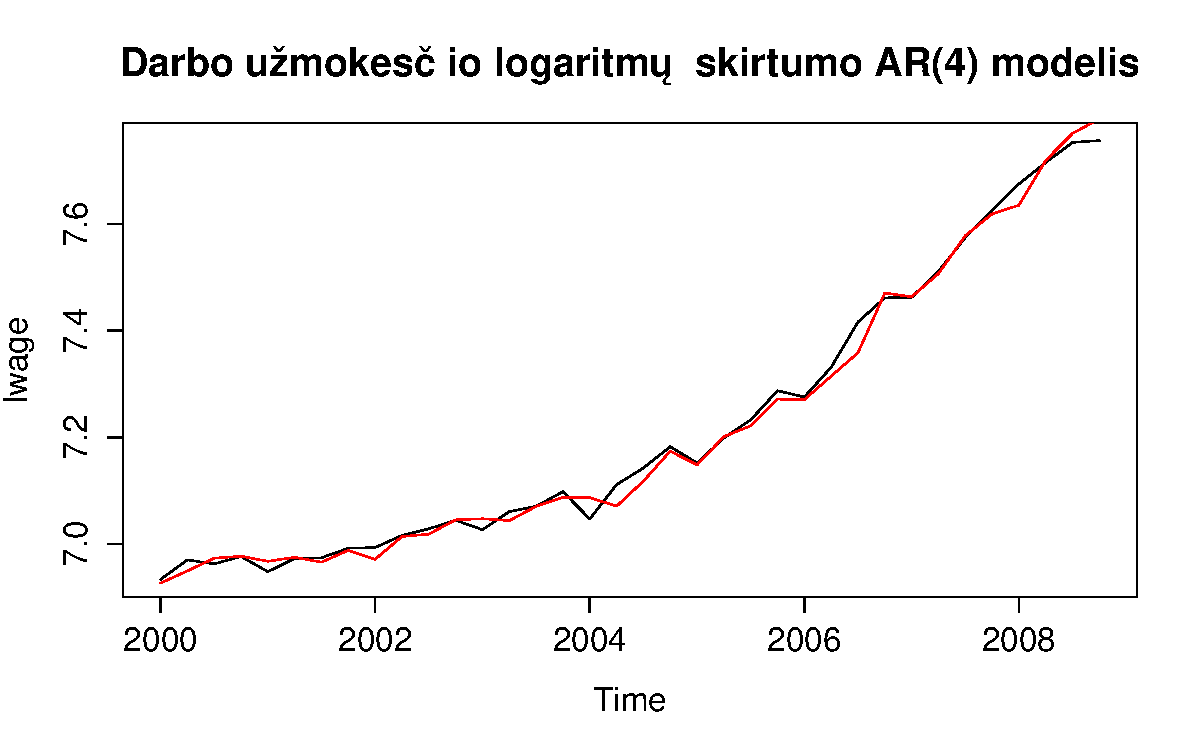
\includegraphics[width=100mm,height=70mm]{arlwage7}
\\ \textit{Paveikslas Nr.3}
\end{center}
\vskip 8pt     
\begin{center}
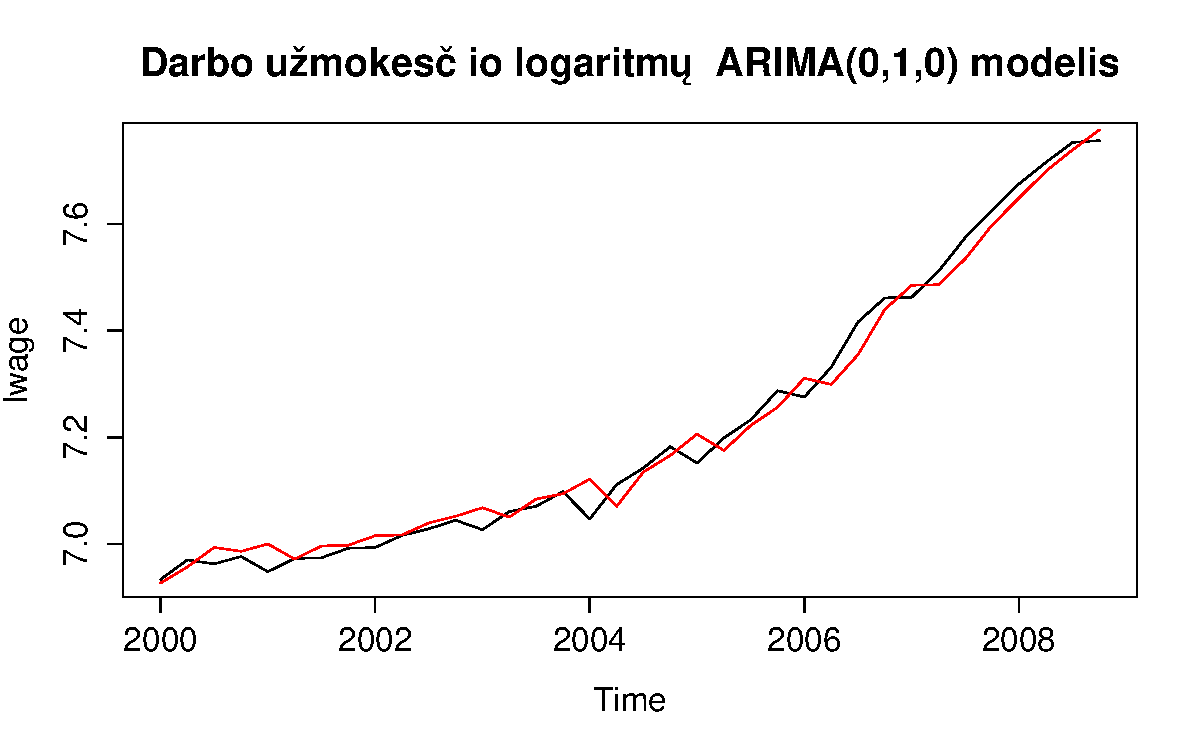
\includegraphics[width=100mm,height=70mm]{arlwage2}
\\ \textit{Paveikslas Nr.4}
\end{center}
\vskip 8pt        
     
$\qquad$ Taigi galutinis autorgresinis modelis, su įvertintais koeficientais yra:
\begin{center}
  \large$ \log wage_t=\log wage_{t-1}+0,081\Delta\log wage_{t-1}+0,104\Delta\log wage_{t-2}-0,031\Delta\log wage_{t-3}+0,755\Delta\log wage_{t-4} $ 
\end{center}  
     
     
     
     
     
     
\subsubsection{Eksponentinis glodinimas} 
\hspace{40pt}Prieš atliekant prognozę ką tik sudarytu autoregresiniu modeliu, ateities reikšmes modeliuosime naudodamiesi eksponentiniu glodinimu. Tai yra vienas sėkmingiausių automatizuoto prognozavimo metodų. Šis metodas remiasi tuo, kad prognozės yra apskaičiuojamos kaip svertiniai vidurkiai praeities reikšmių ir dabartinių reikšmių, suteikiant didesnį svorį dabartinėms reikšmėms. 
\vskip 8pt  
$\qquad$Dabar galime palyginti abiejų modelių 3 metų prognozes: 

\begin{center}
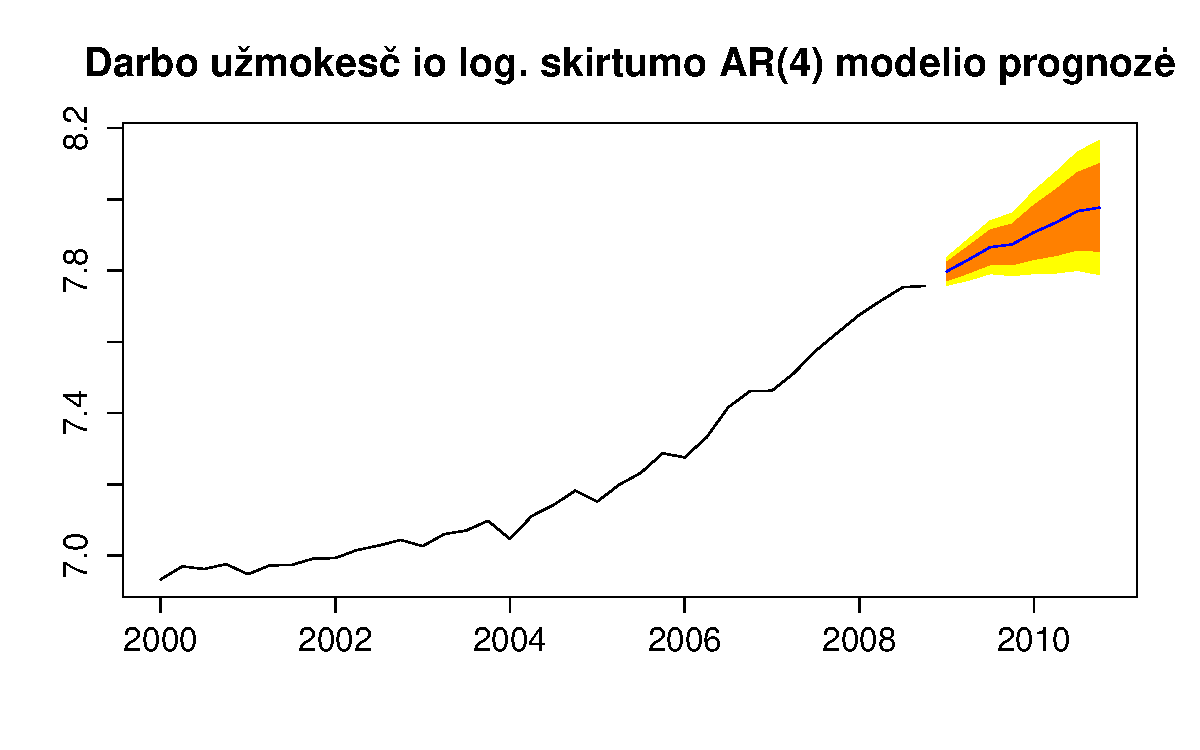
\includegraphics[width=100mm,height=70mm]{farlwage7}
\end{center}

\begin{center}
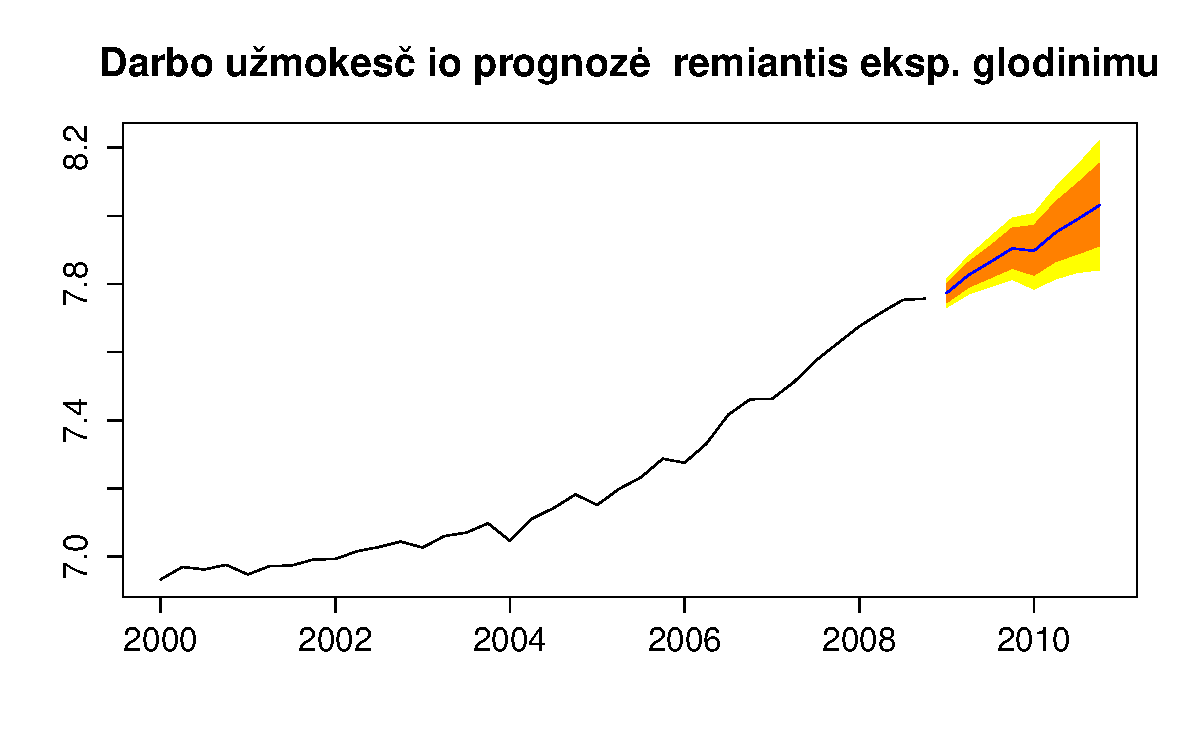
\includegraphics[width=100mm,height=70mm]{fexp}
\end{center}     

\vskip 8pt  
$\qquad$Matome, jog abu modeliai prognozuoja augimą. Tačiau eksponentinis glodinimas prognozuoja staigesnį darbo užmokesčio augimą. 
     
     
     
     
     
     
     
\subsection{ECM}  
\medskip
\hspace{40pt}Korekcijos paklaidų modelis (\textit{angl.} Error Correction Model, \textit{sutr. }ECM) yra dinaminis modelis, kuriame kintamųjų svyravymai kiekviename laiko periode yra susiję su ankstesnių atitinkamų kintamųjų nuokrypiais nuo ilgojo laikotarpio pusiausvyros. 
\vskip 8pt  
$\qquad$Jei kintamieji turi vienetinę šaknį ir jų kointegracijos lygties liekanos nėra stacionarios, tuomet modelis, sudarytas šių kintamųjų lygiams, bus „negeras“, t.y. sudarysime tariamąją regresiją. Modelis turėtų būti sudarytas skirtumams. Tačiau skirtumų regresija apibūdina tik trumpojo laikotarpio sąveiką. 
\vskip 8pt  
$\qquad$Kai kintamieji yra kointegruoti, t.y. kintamieji turi vienetinę šaknį, ir jų kointegracijos lygties liekanos yra stacionarios, paprastas modelis šių kintamųjų skirtumams nebus pakankamai geras. Toks modelis neatkleidžia ilgojo laikotarpio sąryšio tarp kintamųjų. Į modelį būtina įtraukti paklaidų korekcijos narį $ \varepsilon_{t- 1}$. Šis narys yra kintamųjų kointegracijos, kitaip sakant ilgalaikės pusiausvyros  lygties, paklaidų ankstinys. 
\vskip 8pt   
     
\subsubsection{ECM pagal darbo užmokesčio nustatymo mechanizmą}
\hspace{40pt} Taigi, pirmiausia turime sudaryti kointegracijos lygtį. Įtraukdami kintamuosius, remiamės darbo užmokesčio nustatymo mechanizmu. Kointegracijos lygtis yra:
\vskip 8pt      
\begin{center}
\large$ \log wage_t=\alpha' + \kappa'\log p_t + \omega'\log er_t+\upsilon_t $ 
\end{center}    
\vskip 8pt      
$\qquad$Norėdami ištirti, ar šie kintamieji yra kointegruoti, turime ištirti modelio liekanų stacionarumą. Taikydami nuosekliąją procedurą vienetinei šakniai tirti, nustatėme, jog liekanos yra stacionarios. Taigi, kintamieji yra kointegruoti.
\vskip 8pt 
$\qquad$Sekantis žingsnis – ECM sudarymas. Pirmiausia į modelį įtraukiame visų kintamųjų, esančų kointegracijos lygtyje, skirtumus, pasirinkę „protingai“ didelę ankstinių eilę, bei kointegracijos lygties liekanos skirtumo ankstinį, tiksliau:
\vskip 8pt      
\begin{center}
\large$ \Delta \log wage_t = \delta\log t + \lambda \upsilon_{t-1} + \beta_1\Delta \log wage_{t-1}+ \ldots + \beta_4\Delta \log wage_{t-4}+\gamma_0 \Delta \log p_{t}+\ldots +\gamma_4 \Delta \log p_{t-4}+\varphi_0 \Delta \log er_{t}+\ldots +\varphi_4 \Delta \log er_{t-4}+\varepsilon_t$  
\end{center}
kur $ \upsilon_{t-1} $ yra kointegracijos lygties liekanų ankstinys, o $ t $ yra trendas.
\vskip 8pt   
$\qquad$Šis modelis turi nereikšmingų koeficientų prie kai kurių kintamųjų, todėl juos pašalinome iš lygties, palikdami aukščausios eilės reikšmingą ir visus tarpinius ankstinius kiekvienam iš kintamųjų. Po šios procedūros, modelis atrodo taip:     
\vskip 8pt      
\begin{center}
\large$ \Delta \log wage_t =  \lambda \epsilon_{t-1} + \beta_1\Delta \log wage_{t-1}+ \ldots + \beta_4\Delta \log wage_{t-4}+\gamma_0 \Delta \log p_{t}+\ldots +\gamma_4 \Delta \log p_{t-4}+\varphi_0 \Delta \log er_{t}+\varepsilon_t$  
\end{center}

 \begin{center}
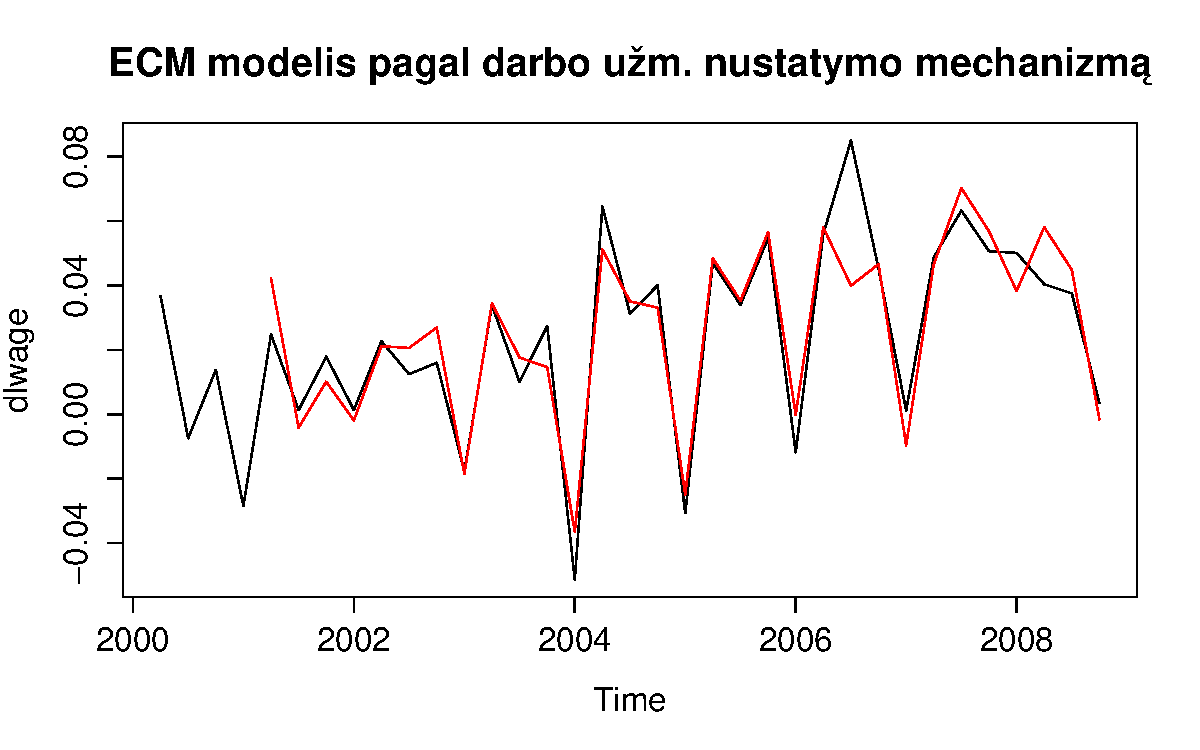
\includegraphics[width=100mm,height=70mm]{ecm12}
\\ \textit{Paveikslas Nr.5}
\end{center}    
     
Remiantis faktinių ir modeliuojamų reikšmių grafiku, galime teigti, jog modelis gana tiksliai aprašo duomenis. Modelį pabandysime patikslinti, įtraukdami darbo našumą.





\subsubsection{ECM įtraukiant darbo našumą}
\hspace{40pt}Remiantis jau pasiūlytais darbo užmokesčio modeliais, bei ekonomine teorija, darbo užmokestis turėtų priklausyti ir nuo darbo našumo. Kuo daugiau pagaminama – tuo didesnis atlyginimas turėtų būti siūlomas, bei reikalaujamas. Todėl sudarysime paklaidų korekcijos modelį įtraukdami darbo našumą. 
\vskip 8pt 
$\qquad$Kointegracijos lygtį papildysime našumo kintamuoju \textit{n}, t.y. 
\vskip 8pt      
\begin{center}
\large$ \log wage_t=\alpha + \kappa\log p_t + \omega\log er_t + \rho\log n_t + \epsilon_t $ 
\end{center} 
\vskip 8pt   
$\qquad$ Šios lygties liekanos yra stacionarios, todėl galime sudaryti paklaidų korekcijos modelį, atliekant analogiškus veiksmus, kaip ankstesnio EC modelio atveju. Dabar pradinis modelis yra:     
     
     
\begin{center}
\large$ \Delta \log wage_t = \delta\log t + \lambda \epsilon_{t-1} + \beta_1\Delta \log wage_{t-1}+ \ldots + \beta_4\Delta \log wage_{t-4}+\gamma_0 \Delta \log p_{t}+\ldots +\gamma_4 \Delta \log p_{t-4}+\varphi_0 \Delta \log er_{t}+\ldots +\varphi_4 \Delta \log er_{t-4}+\psi_0 \Delta \log n_{t}+\ldots +\psi_4 \Delta \log n_{t-4} + \varepsilon_t$  
\end{center}
kur $ \epsilon_{t-1} $ yra kointegracijos lygties liekanų ankstinys, o $ t $ yra trendas.
\vskip 8pt       
$\qquad$Pašalinus nereikšmingus narius analogiškai kaip darėme prieš tai, galutinis modelis yra: 
\begin{center}
\large$ \Delta \log wage_t =  \lambda \epsilon_{t-1} + \beta_1\Delta \log wage_{t-1}+ \ldots + \beta_4\Delta \log wage_{t-4}+\gamma_0 \Delta \log p_{t}+\ldots +\gamma_4 \Delta \log p_{t-4}+\varphi_0 \Delta \log er_{t} + \varepsilon_t$  
\end{center}
  
     
o su skaitinėmis koeficientų reikšmėmis ir išskleistomis kointegracijos lygties liekanomis turime:   



\begin{center}
\large$ \Delta \log wage_t =  -0,43 (\log wage_{t-1}+3,37 - 1,94log p_{t-1} - 1,45\log er_{t-1} - 0,19\log n_{t-1})  + 0,17\Delta \log wage_{t-1}+0,08\Delta \log wage_{t-2}-0,01\Delta \log wage_{t-3} + 0,60\Delta \log wage_{t-4}+1,86 \Delta \log p_{t}-0,86 \Delta \log p_{t-1}+0,14\Delta \log p_{t-2}+0,55\Delta \log p_{t-3} -1,67 \Delta \log p_{t-4}+0,76 \Delta \log er_{t} + \varepsilon_t$  
\end{center}     
 
  \begin{center}
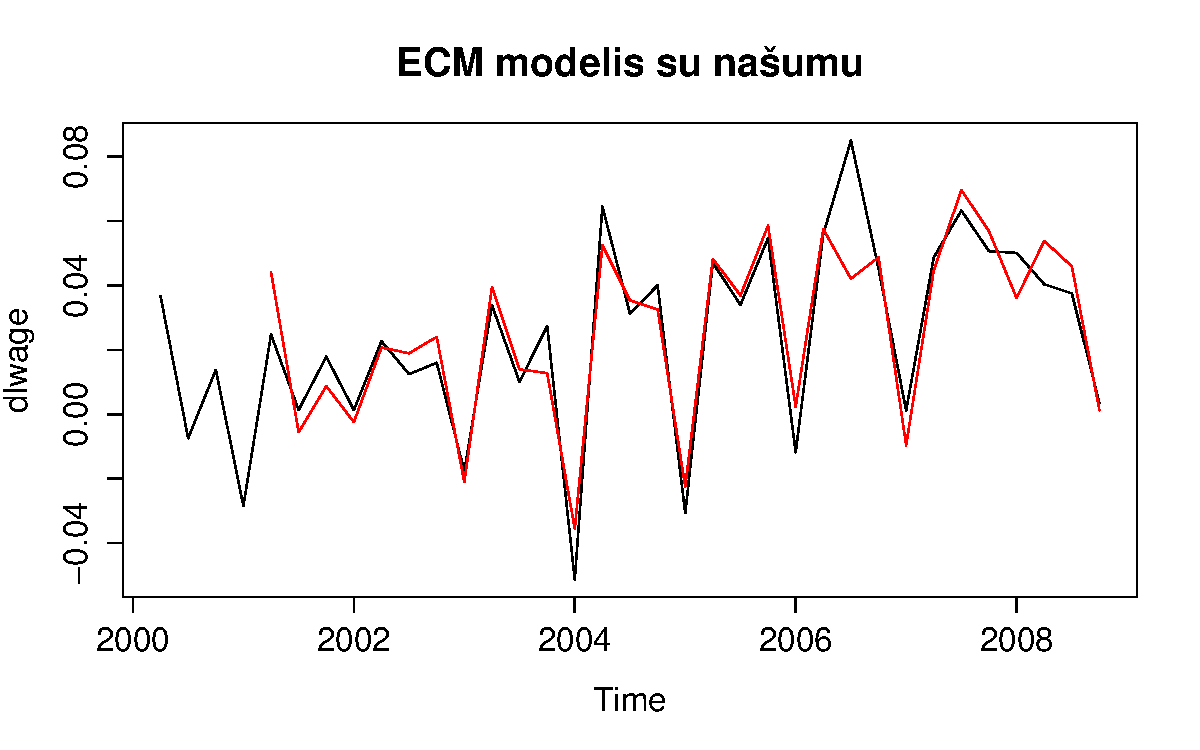
\includegraphics[width=100mm,height=70mm]{ecm23}

\end{center}        
\vskip 8pt
$\qquad$ Šis modelis, lyginant su ECM neįtraukus našumo, yra geresnis. Įtraukus našumą, šio modelio AIC sumažėjo, $ R^2 $  padidėjo. Šios išvados derinasi ir su ekonomikos teorija. 
\vskip 8pt
$\qquad$Koeficientas $ \lambda $, esantis prie kointegracijos lygties paklaidų ankstinio, nusako laiko tarpą, per kurį bus kompensuotas vienetinis nuokrypis nuo pusiausvyros. Paskutiniame modelyje šis koeficeintas lygus -0,43 , tai reiškia, kad vienetinis nuokrypis nuo pusiausvyros bus likviduotas per 1/0,43=2,33 ketvičio. 
\vskip 8pt




\pagebreak
\section{Išvados}
\hspace{40pt}   
Kursinis darbas apima du modelius - autoregresinį modelį ir paklaidų korekcijos modelį. 
\vskip 8pt
$\qquad$Mūsų duomenis geriausiai atitiko ketvirtos eilės autorgresinis modelis logaritmų skirtumams. Tai reiškia, kad Lietuvoje dabartinis darbo užmokesčio pokytis priklauso nuo prieš metus įvykusio darbo užmokesčio pokyčio. Remiantis šio modelio prognozėmis, galime teigti, jog atlyginimų didėjimo tendencija išliks. 
\vskip 8pt
$\qquad$Mes sudarėme du paklaidų korekcijos modelius, iš kurių remiantis įvairiais adekvatumo kriterijais geresnis yra ECM, įtraukus darbo našumą. Remiantis galutiniu modeliu galime daryti išvadą, jog dabartinis darbo užmokesčio pokytis nepriklauso nuo darbo našumo pokyčio, tačiau priklauso nuo jo ankstinio. Darbo užmokestis priklauso nuo dabartinio užimtumo lygio pokyčio, kainų lygio pokyčio ankstinių ir paties darbo užmokesčio ankstinių. Interpretuojant modelio koeficientus, galime teigti, kad didžiausią poveikį darbo užmokesčio pokyčiui daro dabartinis kainų lygio pokytis, bei prieš metus buvusio darbo lygio pokytis. Jei kainų lygis prieš metus padidėja vienu procentu, o kiti kintamieji nekinta, tai darbo užmokestis padidės 1,87 procentais. Taip pat galima teigti, kad darbo užmokesčiui nukrypus nuo pusiausvyros, jis į pusiausvyros lygį sugrįžta per 2,33 ketvirčio. 




\pagebreak     
\section{Literatūra}  

\begin{enumerate}
\item Oliver Blanchard (2007), \textit{Makroekonomika }   
\item Garry Koop (2003), \textit{Data Analysis in Macroeconomics }
\item Svenja Gartner, \textit{ Wages, Inequality and Consequences for the Economy}, Dissertation Plan
\item Vilniaus Universitetas (1991), \textit{Ekonomikos teorija II}
\end{enumerate}





\pagebreak     
\end{document}